\newpage
\subsection{独自考察}
\begin{enumerate}[1.]
	\item 理想変圧器とは以下の条件を満たす変圧器のことをいう\cite{1130000795154912128}.
\begin{itemize}
	\item 巻線の抵抗が0である.
	\item 鉄心の透磁率が無限大であり,したがって磁気回路における磁気抵抗が0である.
	\item 鉄心の鉄損が0である.
	\item 鉄心の磁気飽和は無視できる.
\end{itemize}
\item 一方,実際の変圧器は理想変圧器と異なり,以下のことを考慮しなければならない
\label{real}
\cite{1130154912128}.
\begin{itemize}
	\item 一次及び二次巻線の抵抗や漏れリアクタンスが存在する.
	\item 主磁束を作るために起磁力,すなわち励磁電流が必要である.
	\item 鉄心中に鉄損が存在する.
	\item 鉄心の磁気飽和を無視することは実際上できないが,ここでは特に考慮しない.
\end{itemize}
\item \weq{he}の$\sigma_{h}fB_{m}^{2}=k_{1}\frac{E^{2}}{f}$を示す.
\begin{align*}
	\omega_{h}&=\sigma_{h}fB_{m}^{2}\\
	E&=-N\frac{d\phi_{m}}{d t}\\
	E\sin \omega t&=-N\frac{d}{dt}(\phi_{m} \cos \omega t)\\ 
	&=2\pi f \phi_{m} N\sin \omega t\\
	E&=2\pi f \phi_{m} N\\
	&=2\pi f B_{m} N\\
	B_{m}&=\frac{E}{2\pi f N}\tag{*}\\
	\sigma_{h}fB_{m}^{2}&=\sigma_{h}f\left(\frac{E}{2\pi f N}\right)^{2}\\
	&=\frac{\sigma_{h}E^{2}}{4\pi^{2} f N^{2}}\\
	&=k_{1}\frac{E^{2}}{f}\quad \left(k_{1}\equiv\frac{\sigma_{h}}{4\pi^{2}N^{2}}\right)\\
	\therefore \sigma_{h}fB_{m}^{2}&=k_{1}\frac{E^{2}}{f}
\end{align*}
\item \weq{uzue}の$\sigma_{e}t^{2}f^{2}B_{m}^{2}=k_{2}t^{2}E^{2}$を示す.
\begin{align*}
	\omega_{e}&=\sigma_{e}t^{2}f^{2}B_{m}^{2}\\
	B_{m}&=\frac{E}{2\pi f N}\left((*)より\right)\\
	\sigma_{e}t^{2}f^{2}B_{m}^{2}&=\sigma_{e}t^{2}f^{2}\left(\frac{E}{2\pi f N}\right)^{2}\\
	&=\frac{\sigma_{e}t^{2}E^{2}}{4\pi^{2}N^{2}}\\
	&=k_{2}t^{2}E^{2}\quad \left(k_{2}\equiv\frac{\sigma_{e}}{4\pi^{2}N^{2}}\right)\\
	\therefore \sigma_{e}t^{2}f^{2}B_{m}^{2}&=k_{2}t^{2}E^{2}
\end{align*}
\item モータなどにおける損失は大きく分けて,コアに発生する鉄損,コイル巻線(誘導機の場合は二次導体も含む)に発生する銅損,そして,摩擦や空気抵抗に起因する機械損に分類できる.
さらに,負荷によって導体,鉄に生じる損失のうち鉄損,銅損に含まれないものを漂遊負荷損と呼ぶ.
これらをまとめたものを\wfig{loss_analysis}に示す.
\begin{figure}[h]
	\centering
	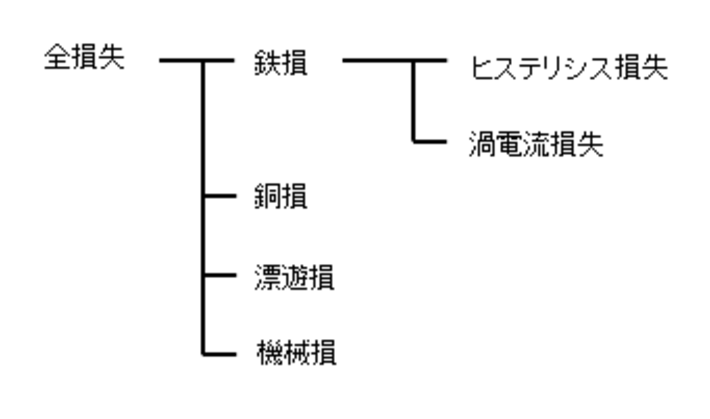
\includegraphics[scale=0.8]{./fig/loss_analysis.pdf}
	\caption{損失の分類\cite{fdls}}
	\label{fig:loss_analysis}
\end{figure}
\end{enumerate}